\documentclass[10pt]{article}
\usepackage[utf8]{inputenc}
\usepackage[T1]{fontenc}
\usepackage{amsmath}
\usepackage{amsfonts}
\usepackage{amssymb}
\usepackage[version=4]{mhchem}
\usepackage{stmaryrd}
\usepackage{bbold}
\usepackage{graphicx}
\usepackage[export]{adjustbox}
\graphicspath{ {./images/} }

\title{Probability and Statistics - Elementary Probability Theory }

\author{Giuliano Casale\\
Department of Computing, Imperial College London}
\date{}


\begin{document}
\maketitle


% \section*{Probability Density Function}
% \begin{itemize}
%   \item Suppose again we have a random experiment with sample space $S$ and probability measure P .
%   \item For a random variable $X: S \rightarrow \mathbb{R}$ we have defined the induced probability
% \end{itemize}

% $$
% \mathrm{P}_{X}(X \leq x)=\mathrm{P}_{X}((-\infty, x])=\mathrm{P}\left(S_{X}\right)=F_{X}(x)
% $$

% \begin{itemize}
%   \item We define the random variable $X$ to be (absolutely) continuous if $\exists f_{X}: \mathbb{R} \rightarrow \mathbb{R}$ such that
% \end{itemize}


% \begin{equation*}
% F_{X}(x)=\int_{u=-\infty}^{x} f_{X}(u) d u \tag{1}
% \end{equation*}


% in which case $f_{X}$ is referred to as the probability density function (pdf) of $X$.

% \section*{Interval Probabilities}
% \begin{itemize}
%   \item What is the probability that a continuous random variable lies in an interval $(a, b]$ ?
%   \item $\mathrm{P}_{X}(a<X \leq b)=\mathrm{P}_{X}(X \leq b)-\mathrm{P}_{X}(X \leq a)$, which in terms of the cdf and pdf gives:
% \end{itemize}

% $$
% \begin{aligned}
% \mathrm{P}_{X}(a<X \leq b) & =F_{X}(b)-F_{X}(a) \\
% & =\int_{a}^{b} f_{X}(x) d x
% \end{aligned}
% $$

% \begin{itemize}
%   \item That is, the area under the pdf curve between $a$ and $b$.\\
% 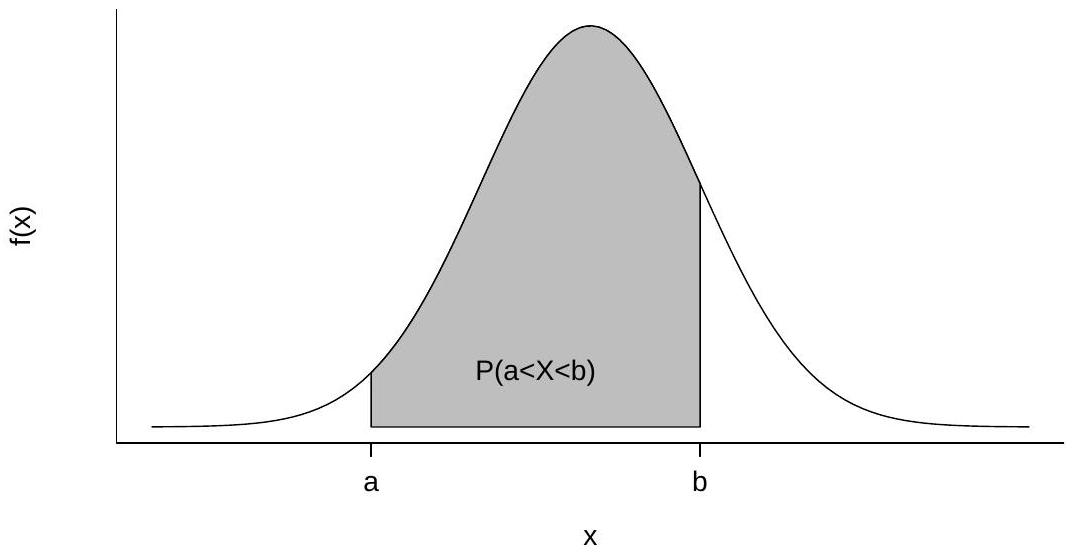
\includegraphics[max width=\textwidth, center]{2025_05_11_1201cfe24e14b364b4ecg-05}
% \end{itemize}

% \section*{Consequences}
% \begin{itemize}
%   \item In the limit $a \rightarrow b$, our definition of interval probability suggests the assignment $\mathrm{P}_{X}(X=b)=0$.
%   \item Consistently with this, the probability assigned to any elementary event $\{x\}, x \in \mathbb{R}$ is zero for a continuous random variable
% \end{itemize}

% $$
% \mathrm{P}_{X}(X=x)=\mathrm{P}_{X}(\{x\})=0 .
% $$

% \begin{itemize}
%   \item Hence, any countable set $\left\{x_{1}, x_{2}, \ldots\right\} \subseteq \mathbb{R}$ will have zero probability measure for a continuous random variable, since $\mathrm{P}_{X}\left(X \in\left\{x_{1}, x_{2}, \ldots\right\}\right)=\mathrm{P}_{X}\left(X=x_{1}\right)+\mathrm{P}_{X}\left(X=x_{2}\right)+\ldots$.
%   \item The support of a continuous random variable must therefore be uncountable - the probabilities could not sum to one otherwise.
% \end{itemize}

% \section*{pdf as the Derivative of the cdf}
% \begin{itemize}
%   \item From Equation (1), we see that the cumulative distribution function (cdf) of a continuous random variable $X$ is
% \end{itemize}

% $$
% F_{X}(x)=\int_{-\infty}^{x} f_{X}(t) d t, \quad \forall x \in \mathbb{R}
% $$

% \begin{itemize}
%   \item Thus, if we are given the cdf of a continuous random variable $X$, we can use the Fundamental Theorem of Calculus to define the pdf of $X$ as
% \end{itemize}

% \section*{Definition}
% $$
% f_{X}(x)=\frac{d}{d x} F_{X}(x) \quad \text { or } \quad F_{X}^{\prime}(x) .
% $$

% \section*{Properties of a pdf}
% \begin{itemize}
%   \item The pdf will always be non-negative, since it is the derivative of the cdf, which is non-decreasing.
%   \item So, in the same way as for cdfs and pmfs of discrete random variables, we have the following checklist to ensure $f_{X}$ is a valid pdf:\\
% (1) $f_{X}(x) \geq 0, \forall x \in \mathbb{R}$;\\
% (2) $\int_{-\infty}^{\infty} f_{X}(x) d x=1$.
%   \item From (1) it is also clear that the pdf (when it exists) of a continuous random variable $X$ completely characterises its distribution, so we often just specify $f_{X}$.
% \end{itemize}

% \section*{Contrast with discrete random variable cdfs}
% \begin{itemize}
%   \item The cdf $F_{X}$ of a continuous random variable $X$ is a non-decreasing function with $F_{X}(-\infty)=0, F_{X}(\infty)=1$ (true for all r.vs.) and also is (absolutely) continuous.
%   \item For a continuous random variable since $\forall x, \mathrm{P}(X=x)=0$, $F_{x}(x)=\mathrm{P}(X \leq x) \equiv \mathrm{P}(X<x)$.
%   \item We do not require $f_{X}(x) \leq 1$, since the pdf $f_{X}(x)$ is not itself a probability, unlike the pmf of a discrete random variable
%   \item For small $h, f_{X}(x) h$ is approximately the probability that takes a value in the small interval, say, $[x, x+h)$.
% \end{itemize}

% \section*{Q\&A: Pareto distribution}
% UNIX process lifetimes follow a so-called Pareto law, with pdf

% $$
% f_{X}(x)=\frac{\alpha k^{\alpha}}{x^{\alpha+1}}
% $$

% with support $x \geq k$, where $k$ is called scale and $\alpha>0$ is called shape.\\
% 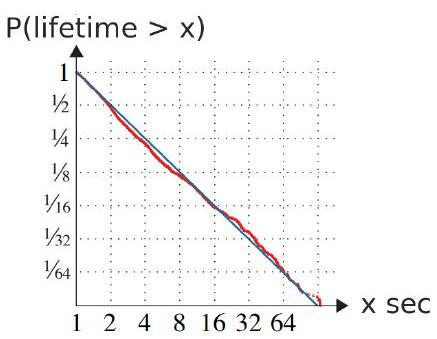
\includegraphics[max width=\textwidth, center]{2025_05_11_1201cfe24e14b364b4ecg-10}

% Q: Determine an expression for the cdf $F_{X}(x)$.\\
% Q: If $X$ models the process lifetime, find $P(X>x)$.

% \section*{Mean, Variance and Quantiles}
% \section*{$\mathrm{E}(X)$}
% For a continuous random variable $X$, we define the mean or expectation of $X$,

% \section*{Definition}
% $$
% \mu_{X} \text { or } \mathrm{E}_{X}(X)=\int_{-\infty}^{\infty} x f_{X}(x) d x
% $$

% More generally, for a function of interest of the random variable $g: \mathbb{R} \rightarrow \mathbb{R}$ we have

% $$
% \mathrm{E}_{X}(g(X))=\int_{-\infty}^{\infty} g(x) f_{X}(x) d x
% $$

% \section*{Linearity of Expectation}
% For continuous random variables, we again have linearity of expectation:

% $$
% \mathrm{E}(a X+b)=a \mathrm{E}(X)+b, \quad \forall a, b \in \mathbb{R},
% $$

% and for two functions $g, h: \mathbb{R} \rightarrow \mathbb{R}$, we have additivity of expectation

% $$
% \mathrm{E}(g(X)+h(X))=\mathrm{E}(g(X))+\mathrm{E}(h(X)) .
% $$

% \section*{$\operatorname{Var}(X)$}
% The variance of a continuous random variable $X$ is given by

% $$
% \sigma_{X}^{2} \text { or } \operatorname{Var}_{X}(X)=\mathrm{E}\left(\left(X-\mu_{X}\right)^{2}\right)=\int_{-\infty}^{\infty}\left(x-\mu_{X}\right)^{2} f_{X}(x) d x
% $$

% Again, it is easy to show that

% $$
% \begin{aligned}
% \operatorname{Var}_{X}(X) & =\int_{-\infty}^{\infty} x^{2} f_{X}(x) d x-\mu_{X}^{2} \\
% & =\mathrm{E}\left(X^{2}\right)-(\mathrm{E}(X))^{2}
% \end{aligned}
% $$

% And for a linear transformation $a X+b$,\\
% $\operatorname{Var}(a X+b)=a^{2} \operatorname{Var}(X), \quad \forall a, b \in \mathbb{R}$.

\section*{Quantiles and percentiles}
\begin{itemize}
  \item The lower and upper quartiles and median of a sample of data are defined as points $\left(\frac{1}{4}, \frac{3}{4}, \frac{1}{2}\right)$-way through the ordered dataset, respectively.
  \item More generally, for a (continuous) random variable $X$ we define the $\alpha$-quantile $Q_{X}(\alpha), 0 \leq \alpha \leq 1$, as the least number satisfying $\mathrm{P}\left(X \leq \mathrm{Q}_{X}(\alpha)\right)=\alpha$, i.e.
\end{itemize}

$$
\mathrm{Q}_{X}(\alpha)=F_{X}^{-1}(\alpha) .
$$

\begin{itemize}
  \item In particular the median of a random variable $X$ is the quantile for $\alpha=\frac{1}{2}$. That is, the solution $x$ to $F_{X}(x)=0.5$.
  \item Similarly, the $k$ th percentile of a distribution is the quantile for $\alpha=k / 100$ (e.g., 95th percentile).
\end{itemize}

\section*{Example: Quartiles, percentiles, quantiles}
\begin{center}
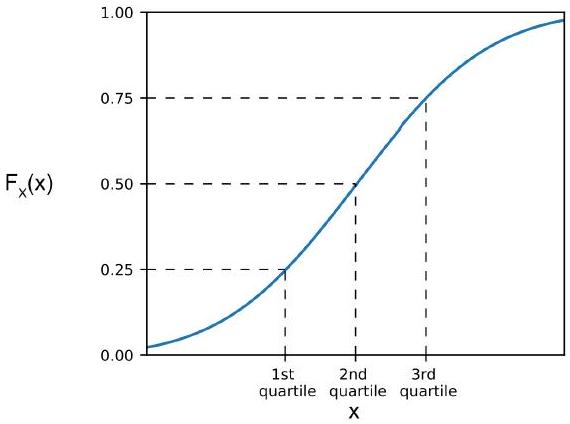
\includegraphics[max width=\textwidth]{2025_05_11_1201cfe24e14b364b4ecg-16}
\end{center}

\begin{itemize}
  \item Lower quartile $=1$ st quartile $=25$ th percentile $=0.25$-quantile.
  \item Median $=2$ nd quartile $=50$ th percentile $=0.50$-quantile.
  \item Upper quartile $=3$ rd quartile $=75$ th percentile $=0.75$-quantile.
\end{itemize}

\section*{Notable Continuous Distributions}
\section*{$\cup(a, b)$}
Uniform Distribution\\
A continuous random variable $X$ with range $(a, b)$ has a uniform distribution on the interval $(a, b)$ if its pdf is

$$
f(x)= \begin{cases}\frac{1}{b-a} & a<x<b \\ 0, & \text { otherwise }\end{cases}
$$

or, equivalently, its cdf is

$$
F(x)= \begin{cases}0 & x \leq a \\ \frac{x-a}{b-a} & a<x<b \\ 1 & x \geq b\end{cases}
$$

We write $X \sim \mathrm{U}(a, b)$.

\section*{Example: U(0,1)}
\begin{center}
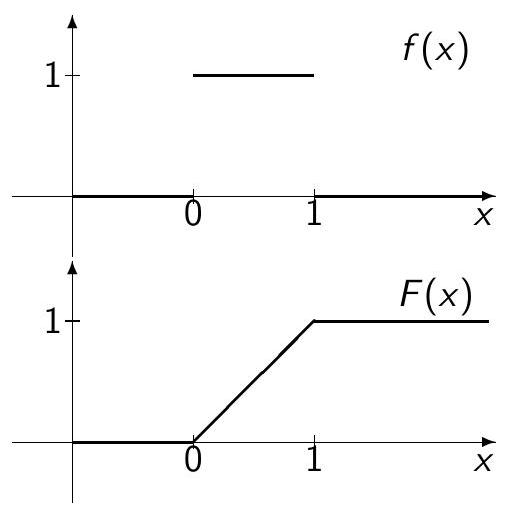
\includegraphics[max width=\textwidth]{2025_05_11_1201cfe24e14b364b4ecg-19}
\end{center}

\section*{Relationship between $U(a, b)$ and $U(0,1)$}
\begin{itemize}
  \item Suppose $X \sim \mathrm{U}(0,1)$, so $F_{X}(x)=x, 0 \leq x \leq 1$.
  \item We wish to map the interval $(0,1)$ to the general interval $(a, b)$, where $a<b \in \mathbb{R}$.\\
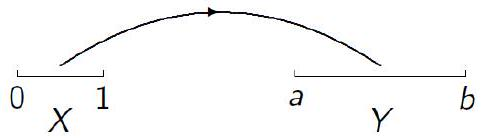
\includegraphics[max width=\textwidth, center]{2025_05_11_1201cfe24e14b364b4ecg-20}
  \item A linear transformation obtains the result: $Y=a+(b-a) X$.
  \item Indeed, it is $Y \sim \mathrm{U}(a, b)$ and\\
$F_{Y}(y)=\mathrm{P}_{Y}(Y \leq y)=\mathrm{P}_{X}\left(X \leq \frac{y-a}{b-a}\right)=F_{X}\left(\frac{y-a}{b-a}\right)=\frac{y-a}{b-a}$
\end{itemize}

\section*{Mean and Variance of $X \sim U(a, b)$}
\begin{itemize}
  \item For the mean
\end{itemize}

$$
\begin{aligned}
E(X) & =\int_{-\infty}^{\infty} x f(x) d x=\int_{a}^{b} x \cdot \frac{1}{b-a} d x=\left[\frac{x^{2}}{2(b-a)}\right]_{a}^{b} \\
& =\frac{b^{2}-a^{2}}{2(b-a)}=\frac{(b-a)(b+a)}{2(b-a)}=\frac{a+b}{2}
\end{aligned}
$$

\begin{itemize}
  \item Similarly for the variance
\end{itemize}

$$
\operatorname{Var}(X)=\mathrm{E}\left(X^{2}\right)-\mathrm{E}(X)^{2}=\frac{(b-a)^{2}}{12}
$$

\begin{itemize}
  \item So
\end{itemize}

$$
\mu=\frac{a+b}{2}, \quad \sigma^{2}=\frac{(b-a)^{2}}{12} .
$$

\section*{Exponential Distribution $\operatorname{Exp}(\lambda)$}
\begin{itemize}
  \item Consider a random variable $X$ with $\operatorname{supp}(X)=[0, \infty)$ and pdf
\end{itemize}

$$
f(x)=\lambda e^{-\lambda x}, \quad x \geq 0
$$

for some $\lambda>0$.

\begin{itemize}
  \item Then $X$ is a exponential (or negative exponential) random variable with rate parameter $\lambda$, and we write $X \sim \operatorname{Exp}(\lambda)$.
  \item Integration between 0 and $x$ leads to the cdf:
\end{itemize}

$$
F(x)=1-e^{-\lambda x}, \quad x \geq 0 .
$$

\begin{itemize}
  \item Moreover, it is possible to show that
\end{itemize}

$$
E(X)=\frac{1}{\lambda} \quad \operatorname{Var}(X)=\frac{1}{\lambda^{2}}
$$

\section*{Example: $\operatorname{Exp}(1), \operatorname{Exp}(0.5) \& \operatorname{Exp}(0.2) p d f s$}
\begin{center}
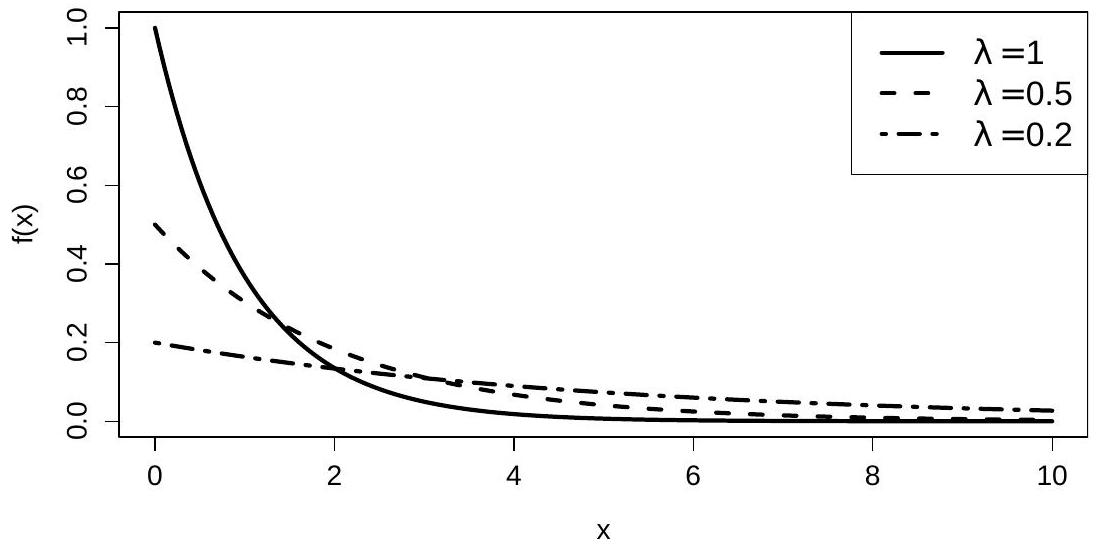
\includegraphics[max width=\textwidth]{2025_05_11_1201cfe24e14b364b4ecg-23}
\end{center}

Probability Density Function\\
Mean, Variance and Quantiles\\
Notable Continuous Distributions\\
Moment generating function

Uniform\\
Exponential\\
Normal\\
Lognormal

\section*{Example: $\operatorname{Exp}(0.2), \operatorname{Exp}(0.5) \& \operatorname{Exp}(1) \mathrm{cdfs}$}
\begin{center}
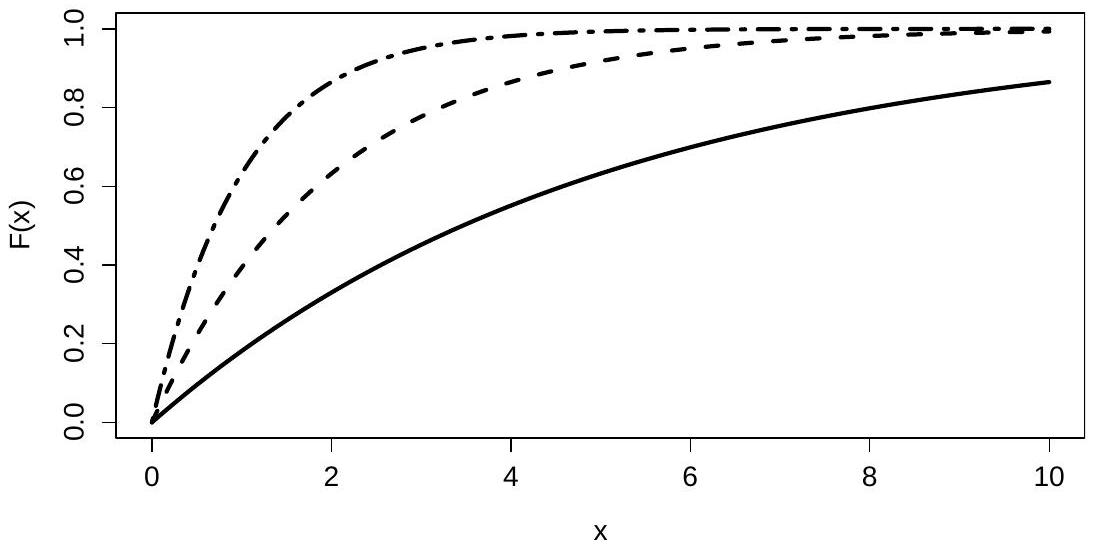
\includegraphics[max width=\textwidth]{2025_05_11_1201cfe24e14b364b4ecg-24}
\end{center}

\section*{Memoryless Property of the Exponential}
\begin{itemize}
  \item The complementary cumulative distribution function (or survival function, or tail distribution) is $\mathrm{P}(X>x)=e^{-\lambda x}$.
  \item An important (and not always desirable) characteristic of the exponential distribution is the so called memoryless or lack of memory property.
  \item To understand the memoryless property, consider the conditional probability $\mathrm{P}(X>x+s \mid X>s)$ for $x, s>0$. When $X$ models time, this is called the distribution of the residual time before the event occurs.
\end{itemize}

\section*{Residual time}
$$
\mathrm{P}(X>x+s \mid X>s)=\frac{\mathrm{P}(X>x+s)}{\mathrm{P}(X>s)} .
$$

\begin{itemize}
  \item Therefore, when $X \sim \operatorname{Exp}(\lambda)$, using the exponential ccdf,
\end{itemize}

$$
\mathrm{P}(X>x+s \mid X>s)=\frac{e^{-\lambda(x+s)}}{e^{-\lambda s}}=e^{-\lambda x}=\mathrm{P}(X>x)
$$

which is again an exponential ccdf with parameter $\lambda$.

\begin{itemize}
  \item So if we think of the exponential random variable as the time to an event, then knowledge that we have waited time $s$ for the event tells us nothing about how much longer we will have to wait - the process has no memory.
\end{itemize}

\section*{Examples}
\begin{itemize}
  \item Exponential random variables are often used to model the time until occurrence of a random event where there is an assumed constant risk, or rate ( $\lambda$ ) of the event happening over time.
  \item So they are frequently used as the "simplest model", for example in queueing theory, reliability analysis and performance modelling.
  \item Examples include:
  \item the time until the next customer arrives at a bank's cashpoint;
  \item the time to failure of a component in a system;
  \item the time until we find the next mistake on my slides;
  \item the distance along a road between potholes;
  \item the time until the next request arrives at a web server.
\end{itemize}

\section*{Link with Poisson Distribution}
\begin{itemize}
  \item Notice the duality between the exponential random variable examples and those we saw for a (discrete) Poisson distribution.
  \item In each case, "number of events" has been replaced with "time between events", or "time to the next event".
\end{itemize}

Claim: If events in a random process occur according to a Poisson distribution with rate $\lambda$ then the time between consecutive events has an exponential distribution with parameter $\lambda$.

\section*{Example: Exponential and Poisson distributions}
\begin{center}
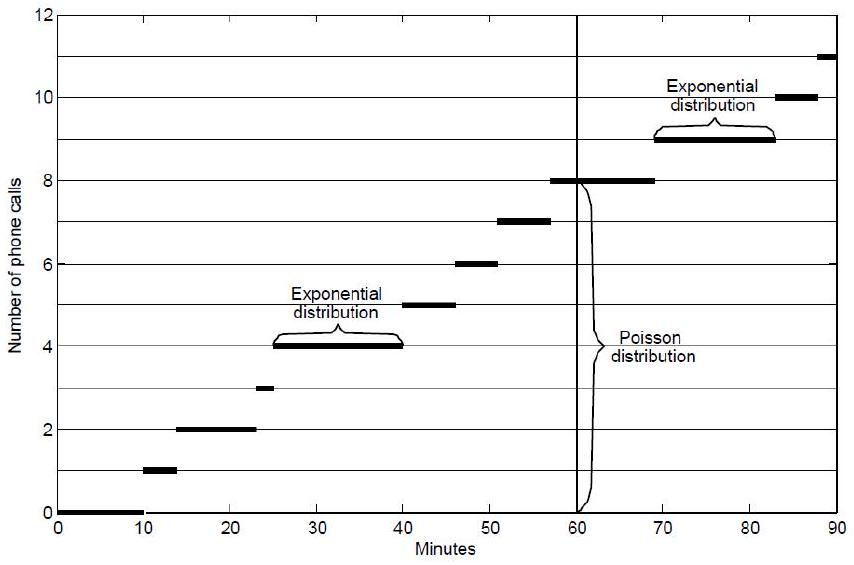
\includegraphics[max width=\textwidth]{2025_05_11_1201cfe24e14b364b4ecg-29}
\end{center}

Source: Taboga

\section*{Proof}
\begin{itemize}
  \item Suppose we have some random event process for which $\forall x>0$, the number of events occurring in $[0, x], N_{x}$, follows a Poisson distribution with mean $\lambda x$, i.e. $N_{x} \sim \operatorname{Poi}(\lambda x)$.
  \item Such a process is known as a homogeneous Poisson process.
  \item Let $X$ be the time until the first event of this process occurs.
  \item Then we have
\end{itemize}

$$
\begin{aligned}
\mathrm{P}(X>x) & \equiv \mathrm{P}\left(N_{x}=0\right) \\
& =\frac{(\lambda x)^{0} e^{-\lambda x}}{0!}=e^{-\lambda x} .
\end{aligned}
$$

\begin{itemize}
  \item Hence $X \sim \operatorname{Exp}(\lambda)$.
  \item A similar argument applies for all subsequent inter-arrival times.
\end{itemize}

\section*{The normal distribution $\mathrm{N}\left(\mu, \sigma^{2}\right)$}
\begin{itemize}
  \item A Normal (or Gaussian) random variable $X$ with range $\mathbb{R}$ has pdf
\end{itemize}

$$
f(x)=\frac{1}{\sigma \sqrt{2 \pi}} \exp \left\{-\frac{(x-\mu)^{2}}{2 \sigma^{2}}\right\}
$$

for some $\mu, \sigma \in \mathbb{R}, \sigma>0$.

\begin{itemize}
  \item Then it can be shown that $X$ has mean $\mu$ and variance $\sigma^{2}$, and we write $X \sim \mathrm{~N}\left(\mu, \sigma^{2}\right)$.
  \item The cdf of $X$ does not have an analytically tractable form for any ( $\mu, \sigma$ ), so we can only write
\end{itemize}

$$
F(x)=\frac{1}{\sigma \sqrt{2 \pi}} \int_{-\infty}^{x} \exp \left\{-\frac{(t-\mu)^{2}}{2 \sigma^{2}}\right\} d t
$$

\section*{Example: $N(0,1), N(2,1) \& N(0,4)$ pdfs}
\begin{center}
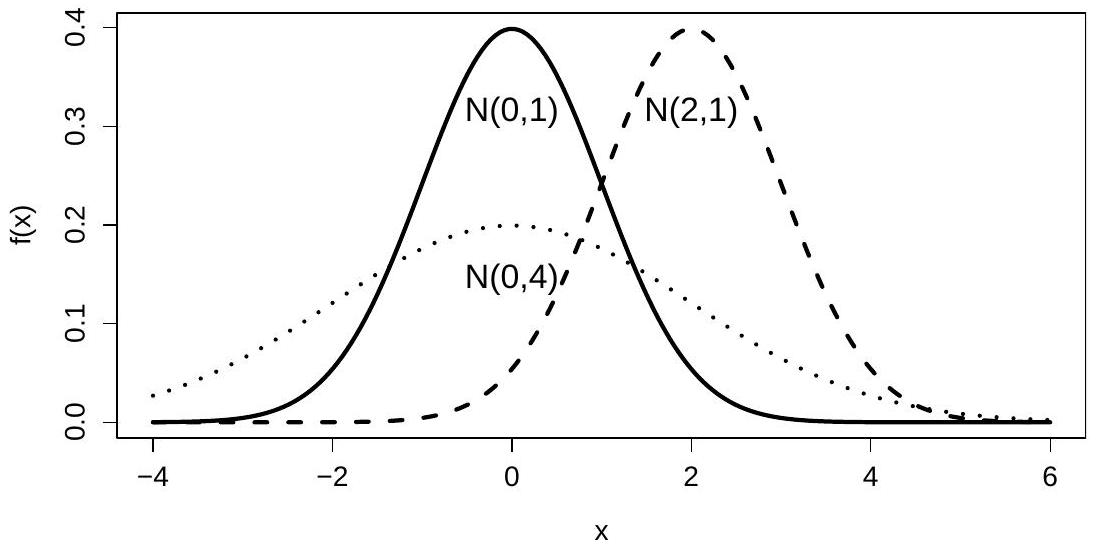
\includegraphics[max width=\textwidth]{2025_05_11_1201cfe24e14b364b4ecg-32}
\end{center}

\section*{Example: $N(0,1), N(2,1) \& N(0,4)$ cdfs}
\begin{center}
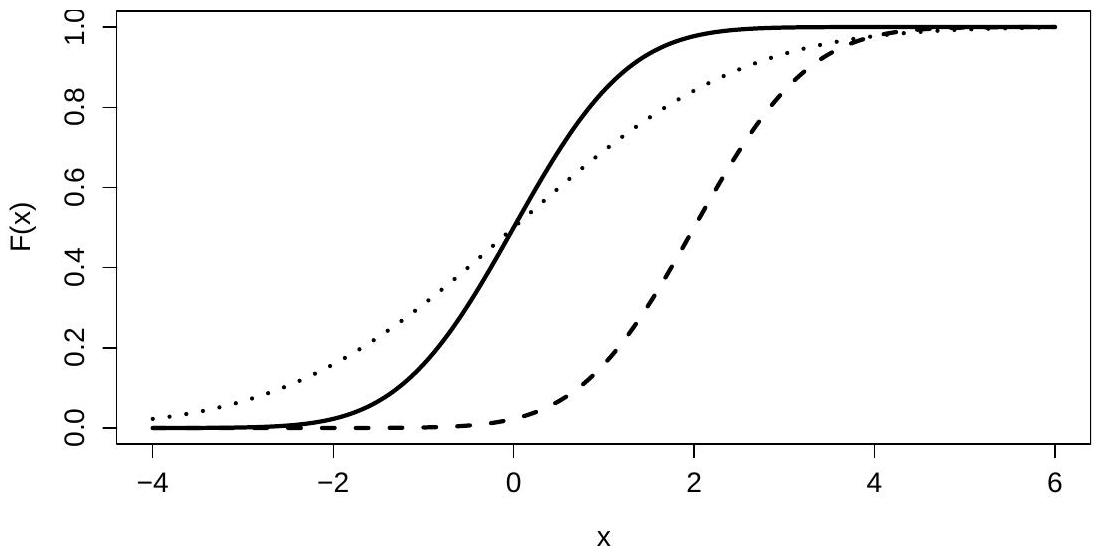
\includegraphics[max width=\textwidth]{2025_05_11_1201cfe24e14b364b4ecg-33}
\end{center}

\begin{itemize}
  \item Setting $\mu=0, \sigma=1, Z \sim \mathrm{~N}(0,1)$ gives the special case of the standard Normal random variable, with simplified pdf
\end{itemize}

$$
f(z) \equiv \phi(z)=\frac{1}{\sqrt{2 \pi}} e^{-z^{2} / 2}
$$

\begin{itemize}
  \item Again for the cdf, we can only write
\end{itemize}

$$
F(z) \equiv \Phi(z)=\frac{1}{\sqrt{2 \pi}} \int_{-\infty}^{z} e^{-t^{2} / 2} d t
$$

\section*{Statistical Tables}
\begin{itemize}
  \item Since the cdf associated with a Normal distribution is not analytically available, numerical integration procedures are used to find approximate probabilities to high accuracy.
  \item In particular, statistical tables contain values of the standard Normal cdf $\Phi(z)$ for a range of values $z \in \mathbb{R}$, and the quantiles $\Phi^{-1}(\alpha)$ for a range of values $\alpha \in(0,1)$.
  \item These were widely used before computers became widely available (pre-1980s).
  \item Linear interpolation is used for approximation between the tabulated values.
  \item All Normal distribution quantiles can be expressed in terms of quantiles from a standard Normal distribution.
\end{itemize}

\section*{Linear Transformations of Normal Random Variables}
\begin{itemize}
  \item Suppose $X \sim \mathrm{~N}\left(\mu, \sigma^{2}\right)$. Then for any constants $a, b \in \mathbb{R}$, $a X+b$ also has a Normal distribution.
  \item More precisely,
\end{itemize}

$$
X \sim \mathrm{~N}\left(\mu, \sigma^{2}\right) \Rightarrow a X+b \sim \mathrm{~N}\left(a \mu+b, a^{2} \sigma^{2}\right), \quad a, b \in \mathbb{R} .
$$

\begin{itemize}
  \item The mean and variance parameters of this transformed distribution follow from the general results for expectation and variance - of any linear function of a random variable.
  \item This allows us to standardise any Normal random variable, i.e.,
\end{itemize}

$$
X \sim \mathrm{~N}\left(\mu, \sigma^{2}\right) \Rightarrow \frac{X-\mu}{\sigma} \sim \mathrm{N}(0,1) .
$$

\section*{Standardising Normal Random Variables}
\begin{itemize}
  \item So if $X \sim \mathrm{~N}\left(\mu, \sigma^{2}\right)$ and we set $Z=\frac{X-\mu}{\sigma}$, then since $\sigma>0$, for any $x \in \mathbb{R}$,
\end{itemize}

$$
X \leq x \Longleftrightarrow \frac{X-\mu}{\sigma} \leq \frac{x-\mu}{\sigma} \Longleftrightarrow Z \leq \frac{x-\mu}{\sigma} .
$$

\begin{itemize}
  \item Therefore we can write the cdf of $X$ in terms of $\Phi$ :
\end{itemize}

$$
\begin{aligned}
F_{X}(x) & =\mathrm{P}(X \leq x)=\mathrm{P}\left(Z \leq \frac{x-\mu}{\sigma}\right) \\
& =\Phi\left(\frac{x-\mu}{\sigma}\right)
\end{aligned}
$$

\section*{Table of $\Phi$}
\begin{center}
\begin{tabular}{|l|l|l|l|l|l|l|l|}
\hline
$z$ & $\Phi(z)$ & $z$ & $\Phi(z)$ & $z$ & $\Phi(z)$ & $z$ & $\Phi(z)$ \\
\hline
0 & . 500 & 0.9 & . 816 & 1.8 & . 964 & 2.8 & . 997 \\
\hline
. 1 & . 540 & 1.0 & . 841 & 1.9 & . 971 & 3.0 & 998 \\
\hline
. 2 & . 579 & 1.1 & . 864 & 2.0 & . 977 & 3.5 & 9998 \\
\hline
. 3 & . 618 & 1.2 & . 885 & 2.1 & . 982 & 1.282 & . 900 \\
\hline
. 4 & . 655 & 1.3 & . 903 & 2.2 & . 986 & 1.645 & . 950 \\
\hline
. 5 & . 691 & 1.4 & . 919 & 2.3 & . 989 & 1.96 & 975 \\
\hline
. 6 & . 726 & 1.5 & . 933 & 2.4 & . 992 & 2.326 & 990 \\
\hline
. 7 & . 758 & 1.6 & . 945 & 2.5 & . 994 & 2.576 & . 995 \\
\hline
. 8 & . 788 & 1.7 & . 955 & 2.6 & . 995 & 3.09 & 999 \\
\hline
\end{tabular}
\end{center}

\section*{Using Table of $\Phi$}
\begin{itemize}
  \item $\Phi(z)$ has been tabulated for $z>0$ only because the standard Normal pdf $\phi$ is symmetric about 0 , so $\phi(-z)=\phi(z)$.
  \item For the cdf $\Phi$, this means
\end{itemize}

$$
\Phi(z)=1-\Phi(-z) .
$$

\begin{itemize}
  \item So, for example, $\Phi(-1.2)=1-\Phi(1.2) \approx 1-0.885=0.115$.
  \item Similarly, if $Z \sim \mathrm{~N}(0,1)$ and we want $\mathrm{P}(Z>z)$, we use
\end{itemize}

$$
\mathrm{P}(Z>z)=1-\Phi(z)=\Phi(-z) .
$$

\begin{itemize}
  \item For example,
\end{itemize}

$$
\mathrm{P}(Z>1.5)=1-\mathrm{P}(Z \leq 1.5)=1-\Phi(1.5) \quad(=\Phi(-1.5))
$$

\section*{Important Quantiles of $\mathrm{N}(0,1)$}
\begin{itemize}
  \item We will often have cause to use the $97.5 \%$ and $99.5 \%$ quantiles of $N(0,1)$, given by $\Phi^{-1}(0.975)$ and $\Phi^{-1}(0.995)$, respectively.
  \item $\Phi(1.96) \approx 97.5 \%$.
\end{itemize}

So with $95 \%$ probability an $N(0,1)$ random variable will lie in the range $[-1.96,1.96]$

\begin{itemize}
  \item $\Phi(2.58)=99.5 \%$.
\end{itemize}

So with $99 \%$ probability an $\mathrm{N}(0,1)$ random variable will lie in the range [-2.58, 2.58].

\section*{Lognormal Distribution}
Suppose $X \sim \mathrm{~N}\left(\mu, \sigma^{2}\right)$, and consider the transformation $Y=e^{X}$.

\begin{itemize}
  \item It can be shown that the random variable $Y$ has density
\end{itemize}

$$
f_{Y}(y)=\frac{1}{\sigma y \sqrt{2 \pi}} \exp \left[-\frac{\{\log (y)-\mu\}^{2}}{2 \sigma^{2}}\right], \quad y>0
$$

\begin{itemize}
  \item $Y$ is said to follow a lognormal distribution.
  \item Used a lot in financial modelling and to describe "heavy tailed" distributions.
\end{itemize}

% \section*{Moment generating function}
% \section*{Moment generating function, $M_{X}(t)$}
% \begin{itemize}
%   \item We close the study of basic random variables illustrating two alternative methods to describe a distribution.
%   \item The moment generating function (mgf) $M_{X}(t)$ of a (continuous) random variable $X$, is defined by
% \end{itemize}

% $$
% M_{X}(t)=\mathrm{E}\left(e^{t X}\right)=\int_{-\infty}^{\infty} e^{t x} f_{X}(x) d x
% $$

% \begin{itemize}
%   \item The mgf can be defined also for a discrete random variable $X$ as
% \end{itemize}

% $$
% M_{X}(t)=\mathrm{E}\left(e^{t X}\right)=\sum_{x_{i} \in \operatorname{supp}(X)} e^{t x_{i}} p\left(x_{i}\right)
% $$

% where $p(x)$ is the pmf of $X$.

% \section*{Obtaining moments from the mgf}
% \begin{itemize}
%   \item Assuming differentiation inside the expectation operator (or integral) is valid, the mgf provides an alternative way to obtain moments
% \end{itemize}

% $$
% E\left[X^{n}\right]=\left.\frac{\mathrm{d}^{n} M_{X}(t)}{\mathrm{d} t^{n}}\right|_{t=0}
% $$

% \section*{Characteristic function, $\phi_{X}(t)$}
% \begin{itemize}
%   \item The integral that defines the mgf may not exist. In these cases, we may use instead the characteristic function
% \end{itemize}

% $$
% \phi_{X}(t)=M_{X}(i t)=\int_{-\infty}^{\infty} e^{i t x} f_{X}(x) d x
% $$

% where $i=\sqrt{-1}$ is the imaginary unit.

% \begin{itemize}
%   \item Unlike the mgf, the characteristic function $\phi_{X}(t)$ exists always.
%   \item Moments can be derived in a similar way
% \end{itemize}

% $$
% E\left[X^{n}\right]=\left.i^{-n} \frac{\mathrm{~d}^{n} \phi_{X}(t)}{\mathrm{d} t^{n}}\right|_{t=0}
% $$

\section*{Product of Independent Random Variables}
\begin{itemize}
  \item Consider two independent random variables $Z_{1}$ and $Z_{2}$.
  \item Setting $Z=\left(Z_{1}, Z_{2}\right)$, what can we say about the expectation of the random variable $g(Z)=Z_{1} Z_{2}$ ?
  \item Upon studying joint random variables, we will be able to show that, due to independence
\end{itemize}

$$
E\left[Z_{1} Z_{2}\right]=E\left[Z_{1}\right] E\left[Z_{2}\right]
$$

\begin{itemize}
  \item The result generalizes as $E\left[\prod_{i=1}^{n} Z_{i}\right]=\prod_{i=1}^{n} E\left[Z_{i}\right]$.
\end{itemize}

\section*{Sum of Independent Random Variables}
\begin{itemize}
  \item A consequence of the previous result is that the mgf of the sum of independent r.vs. is the product of their mgfs, e.g.:
\end{itemize}

$$
\begin{aligned}
M_{Z_{1}+Z_{2}}(t) & =\mathrm{E}\left(e^{t\left(Z_{1}+Z_{2}\right)}\right)=\mathrm{E}\left(e^{t Z_{1}} e^{t Z_{2}}\right) \\
& =\mathrm{E}\left(e^{t Z_{1}}\right) \mathrm{E}\left(e^{t Z_{2}}\right)=M_{Z_{1}}(t) M_{Z_{2}}(t)
\end{aligned}
$$

More generally, for a sum of $n$ independent r.vs. $S_{n}=\sum_{j=1}^{n} X_{j}$ we have then:

$$
M_{S_{n}}(t)=\prod_{j=1}^{n} M_{X_{j}}(t)
$$


\end{document}